\subsection{Data Processing Pipeline}
\label{subsec:pipeline}

The following chapters showing the used data sources and architecture which we used to solve our task described in \fullref{subsec:usecase}
After \fullref{subsubsec:architecture} we explain the technical setup which we used to implement our data processing pipeline as well as
our approach for \textit{Data Ingestion}, \textit{Data Storing} and \textit{Data Cleaning} to get the data ready for analysis.
Finally, we explain which measures we implemented to clean up the data for analysis.

\paragraph{Data sources}
\label{subsec:Data sources}
As mentioned previously, a lot of various key figures were collected for the following data analysis relating to the restaurant business. The main data source with helpful key figures should be at least from one restaurant online review website. In this case the online platform of yelp was chosen. yelp is a popular community site that allows restraurants to present themselves, give visitors a star scale rating of one to five, or give visitors the opportunity to leave comments. For example, the interface Yelp Fusion provides the name of the restaurant, the type of food or the coordinates of the restaurant with latitude and longitude.
\newline
In addition to this some other datasets relating to Germany's cities were used for the data analysis:
\begin{itemize}
\item CSV file with the population and the area
\end{itemize}
\newline
Purchasing power is an important factor in the catering industry. It makes little sense to open a three-star restaurant in a social focus area or vice versa. A fast food business will not last long between high-end haute cuisine restaurants. In 2016, public television broadcast a study on the quality of life in Germany. These studies included different population, city, and quality reports, with reference to external sources. One of the studies contained information on purchasing power in the cities of Germany. The report led to an external provider who had published this survey \cite{BuyingPower}. This evaluation was publicly available in the download portal of the website in portable document format and was very well suited to adapting this with a python converter in the postgres database. This attribute complements the model to determine the price level for a restaurant.
\newline
For our use case and in general, it is absolutely necessary to know how much rent you can pay in the month or year or whether you can afford a property. In search of a rent index in Germany, we first came across an open-source evaluation in .json format \cite{Sparda}. Unfortunately, this was only the average land prices. Thereupon the possibility opened by an interface to real estate platforms \cite{ImmoScout} to get more accurate and more up-to-date rental and land prices.

\subsubsection{Architecture}
\label{subsubsec:architecture}
In order for our project, described in \fullref{subsec:usecase}, to succeed, it is of inestimable value to have a
architecture that supports this in the best possible way.

The requirements for our architecture are as follows:
\begin{enumerate}
  \item Multiple data sources must be supported.
  \item All data collected must be stored in its original representation to be able to answer still unknown questions at a later point in time.
  \item The areas of data acquisition, analysis and visualization must be separated.
\end{enumerate}

When dealing with large amounts of data, the following two architectural approaches distinguish between each other:

\paragraph{Lambda Architectur}
Named after the Greek $\lambda$, this approach is characterized by the fact that the streaming data is processed in two ways.
On the one hand, the data stream is routed directly to a \textit{Speed Layer}, which is often based on in-memory technology,
processes it in real time and makes it available to the \textit{Serving Layer}.
Since streams are by definition infinite and the speed layer is expensive and physically finite,
the stream is routed from \textit{Ingestion Layer} into the \textit{Batch Layer} in parallel.
This layer stores the data persistently and starts a batch job after a defined interval to process the started data and transfer it to the serving layer.
So it is the responsibility of the serving layer to mix the aggregated inventory data from the batch layer with the real-time data of the speed layer,
which has not yet been processed by the batch layer.\cite{lambda} \cite{jaxkappa}

\begin{figure}[h]
	\centering
	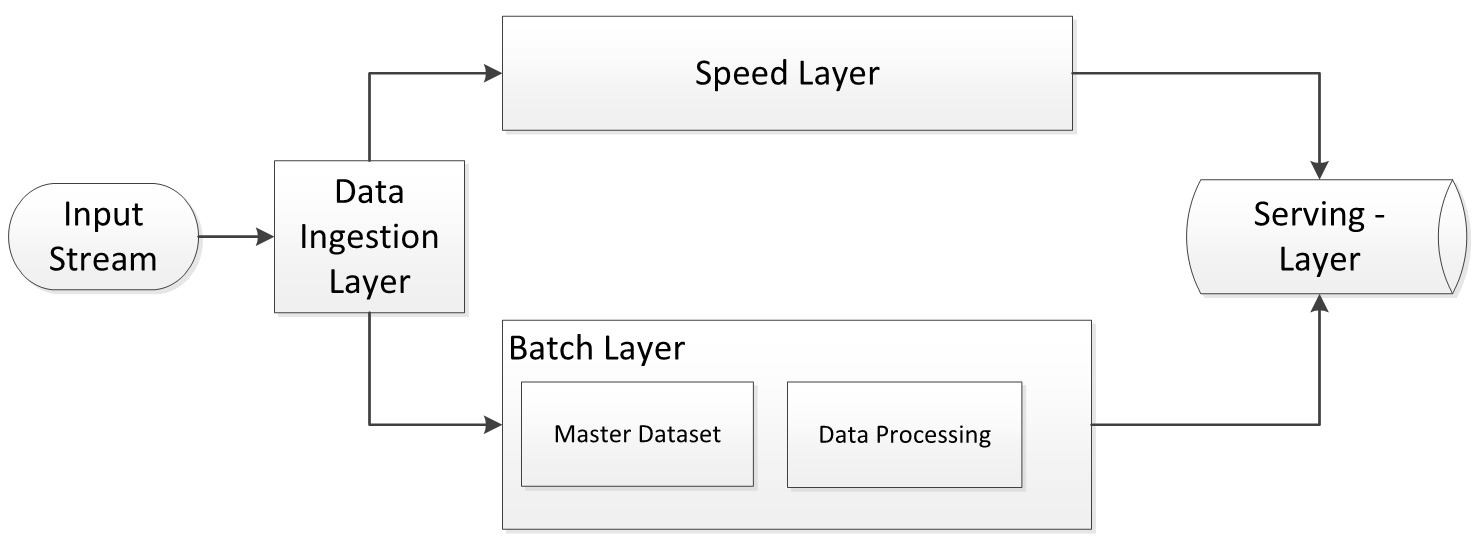
\includegraphics[width=10cm]{berle_lambda-architektur_3.jpg}
	\caption[Scheme of $\lambda$ architecture]{Scheme of $\lambda$ architecture\cite{jaxkappa}}
	\label{fig:KafkaArchitecture}
\end{figure}

\paragraph{Kappa Architectur}
This approach, designed by Confluent co-founder and CEO Jay Kreps, dispenses with batch processing and therefore only requires
\textit{Ingestion-}, \textit{Speed-} and \textit{Serving-Layer}.
This saves the development and operation of two separate layers and the time-consuming mixing of batch data with live data in the \textit{Serving-Layer}.
A prerequisite, however, is that the \textit{Ingestion-Layer} does not only pass through data volatilely,
but rather holds the raw data persistently in the \textit{Master-Dataset} as a \textit{Buffer} in order to make the raw data available again in case of a new,
not yet precalculated request or change in the \textit{Speed-Layer}.
To ensure a correct replay of the messages, the buffer is based on a canonical log, in which only messages can be added unchanged, but already saved messages can no
longer be changed or moved in their order.
This approach was named after the Greek $\kappa$ in order to illustrate both proximity and demarcation to the $\lambda$ architecture.
\cite{Kappa} \cite{Kappa2}

\begin{figure}[h]
	\centering
	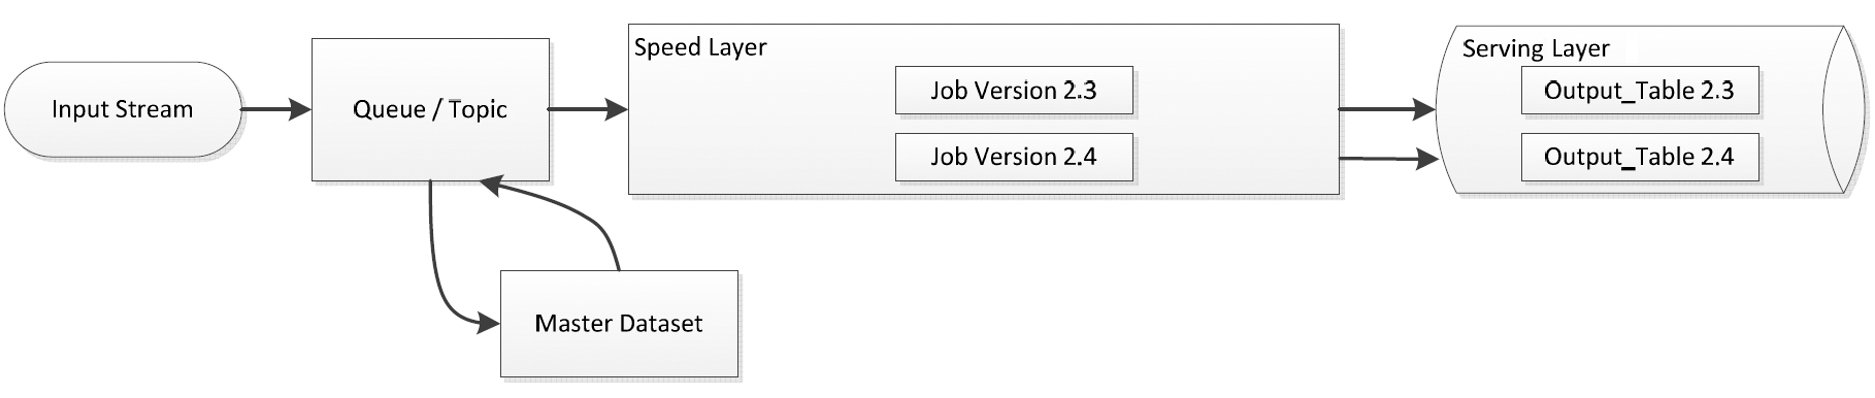
\includegraphics[width=10cm]{berle_lambda-architektur_4.jpg}
	\caption[Scheme of $\kappa$ Architectur]{Scheme of $\kappa$ Architectur\cite{jaxkappa}}
	\label{fig:KappaArchitecture}
\end{figure}

Both the Kappa and the Lamba architecture cover our requirements.
Via the input stream, any number of data sources can be accessed, in the
data ingestion layer, all collected data is stored, and then the data is processed and can be persisted in the serving layer.
The analysis part can now be executed on the serving layer.
The separation into different layers also fulfils our third requirement.

% TODO: kann das so stehen bleiben?
As explained in chapter \fullref{subsubsec:sources} our biggest data source is the Fusion \ac{API} of Yelp and
the Search \ac{API} of ImmobilienScout24.
Due to the fact that Yelp data - with the exception of the Business ID - may not be stored for more than 24 hours,\cite{YelpFaq}
the amount of data collected is manageable.

Due to the manageable amount of data that should be available to us in the end and the limited time period to complete this project,
we consciously forgo a batch layer and therefore also the Lambda architecture
in order not to unnecessarily increase the complexity of our architecture but also to reduce the processing time of data at the same time.
So we decided for a simplified version of the Kappa architecture.

In step 1 we collect the data from different data sources and write them unchanged into \gds{}
The second step consists of transporting the data into the \pg{} database from where it can be analyzed later on.
The transport included not only the simple moving of the data from the source to the target database but also the conversion of the data
into a format that has been adapted to the relational database.
Conversion, in this case, does not only mean to add additional attributes to enrich the subsequent analysis and visualization in a more meaningful way,
but also sorting out not used attributes.
The last step, the analysis of the data, was done depending on the scenario either with the Bi- and Software Analysis Software Tableau or with a Python Script and the libraries \code{pandas} and \code{matplotlib}.
\newline
The following picture shows our previously described variant of the Kappa architecture.

%TODO: picture

\subsubsection{Technical Setup}
\label{subsubsec:setup}
The Kappa architecture was realized in the programming language Python (version 3.6).
The following Python libraries were additionally installed:
\begin{itemize}
  \item \code{google-cloud-datastore}
  \item \code{sqlalchemy}
  \item \code{psycopg2}
  \item \code{requests}
  \item \code{requests\_oauthlib}
\end{itemize}
Furthermore for connecting the Yelp Fusion \ac{API} we used the python implementation of the Yelp Fusion client on GitHub\footnote{\url{https://github.com/Yelp/yelp-fusion}}
We extended this python module by our own requirements and wishes.
\newline
For the \textit{Data Cleaning} part we also wrote our own python scripts as well as some \ac{SQL} statements which we directly executed on the \pg{}.

\subsubsection{The Factory Pattern}
\label{subsubsec:factory}
As explained in \fullref{subsubsec:sources} we have different data sources from which the required data must be retrieved.
For this reason it is extremely important that our program is written in such a way that new data sources can be connected at any time.
This was realized by a combination of dynamic programming and a simple \textit{Factory Pattern}\footnote{\url{https://en.wikipedia.org/wiki/Factory_method_pattern}}.
By using the factory pattern we can abstract from the implementation logic and quickly and easily connect new data sources to the existing logic without changing anything in the underlying process.

The part of the program that is responsible for collecting and storing the data in \gds{}, is called \textbf{collector}
and that part that is responsible for transporting and mapping the raw data into \pg{} is called \textbf{transporter}
There are two modules that realize the factory pattern for both collector and transporter:

\begin{itemize}
  \item \code{factory.py}
  \item \code{creator.py}
  \item \code{collector.py}
  \item \code{transporter.py}
\end{itemize}

The module \code{factory.py} contains both the class \code{AbstractFactory}, which is an abstract variant of a concrete factory, and the class
\code{EverythingFactory} which inherits from the \code{AbstractFactory} and instantiates concrete classes of \code{collector.py} and \code{transporter.py}.
with help of the \code{creator.py} module.
This auxiliary class in this module consists of several static methods which create and return an instance of a \textit{collector}/\textit{transporter} instance.

\subsubsection{Data Ingestion}
\label{subsubsec:ingestion}
As descriped in\cite{ingestion} \textit{Data Ingestion} is the process of obtaining and importing data for immediate use or storage in a database.
In our usecase we are collecting data from various data sources, thus we need different implementation approaches on each kind of datasource.
\newline
Across all \code{collectors} data were collected from a total of five different types of data sources:
\begin{itemize}
  \item \ac{JSON}
  \item \ac{API}
  \item \ac{PDF}
  \item \ac{CSV}
  \item Web
\end{itemize}
A part that should not be underestimated is the resulting quality of the data.
While \ac{API}, \ac{CSV} and \ac{JSON} files consist of very structured data and reading them does not require much effort,
data from a \ac{PDF} file or homepage are unstructured and require a higher implementation effort and possibly an additional
\textit{Data Cleaning} step is required before using them in the analysis part to get the results that are truly reflecting the reality.
% For the implementation of \textit{Data Ingestion} the \code{collector.py} module was developed.
% Within this module is the base class for the flow logic of the concrete \textit{collectors}.
% Due to the inhomogeneity of the data sources and the associated different logic per \textit{collector}, the \code{Collector} class only contains the logic
% to store a newly created entity in the \gds{} and other auxiliary methods.
% That means that it is not possible to implement the flow logic in the base class, but be implemented to a large extent in each subclasses.
%
% To realize the \textbf{collector} and its subclasses the Python library \code{google-cloud-datastore} is used.
% The library \code{google-cloud-datastore} is a client with which it is possible to perform all known \ac{CRUD} operations for the \gds{}.

\subsubsection{Data Storage}
\label{subsubsec:storage}
In order for the data to be available for analysis and visualization, it must be read from the \gds{} and imported into the \pg{} database.
Before the data in the \pg{} can be personalized, it must be mapped to the respective table format.

This process is called \textit{Data Storage} and the Python module \code{transporter.py} was developed especially for this purpose.
In contrast to the implementation of the \code{collector} module, a large part of the \textit{Data Storage} logic is in the base class.
Only the logic for transforming the \gds{} entity to a \pg{} database table must be implemented as soon as a new
data source is to be connected.

In summary, the following steps had to be taken to develop a new \textit{transporter}:
\begin{itemize}
  \item Create a new \pg{} table with \code{sqlalchemy}
  \item  Create a new \code{<example>\_transporter.py} file that inherits from the base class.
  \item Implementation of the \code{map()} Methdode in which the \gds{} entity is received and one or more \code{sqlalchemy} object(s) are created and returned.
\end{itemize}

\subsection{Data Cleaning}
\label{subsec:cleaning}
The quality of data can be described in many dimensions like \eg{} the trustworthiness of the data source, the consistency of the data,
or their accuracy as well as their topicality. % Quelle aus PDF
Just with very unstructured data, as in our case the collected dishes from the web page speisekarte.de, the cleaning of the data is
inevitable to get a good and accurate analysis result.
However, even with supposedly good data sources such as \acp{API}, there may be errors in the data.
such as \eg{} the mixing of different languages or the lack of information.
Differences in data quality can also occur in the process of data collection.
\newline
This paragraph explains the measures taken in this project to clean up the data collected.
\paragraph{Review Count Cleaning}
In the \pg{} database the review\_count of some restaurants was assigned the value \code{NULL}.
If a new comparison with the \ylp{} \ac{API} did not result in a change of the review count,
this \code{NULL} value was replaced by the number 0.
\paragraph{Address Cleaning}
The \ac{API} of \ylp{} is designed so that an HTTP code 403 or 404 will be transmitted if no address to a restaurant
can be found.
With a python script the \ylp{} \ac{API} was addressed again to find the restaurant's address.
If still no city or postcode was found for this restaurant, this restaurant was deleted for reasons of simplicity,
since a restaurant without a postcode or city has no use for the subsequent analysis.
\paragraph{Price Range Cleaning}
In the price\_range attribute there were occasional occuring \code{NULL} values which possibly could be filled when addressing the \ylp{} \ac{API} a second time.
If this was not the case, the \code{NULL} values were filled with the mode of the price\_range from the current city.
\paragraph{City Cleaning}
Despite the fact that the \code{city} attribute of a restaurant always came from Yelp it came to a mixture of the German and English language,
so we translated the english names in its german counterparts manually.
Furthermore, the German city ''Frankfurt am Main'' was available in different spellings.
However, this could be fixed with a simple \ac{SQL} statement.
\paragraph{Buying Power Cleaning}
The data source found for acquiring the buying\_power for various german cities unfortunately contained not the buying\_power for all german cities.
We solved this isssue by replacing, the missing buying\_power with the average buying\_power in Germany in order to be able to carry out at least a rough analysis.
\paragraph{Average Purchase Price Cleaning}
Also with the average purchase price of a restaurant per m\textsuperscript{2} the original data source did not include all cities of Germany and therefore
some \code{NULL} values remained in the database.
These have been replaced with the Germany-wide average.
\paragraph{Menu Item Cleaning}
Although most of the cleaning took place after the persistence of the data in the database, the various dishes on a menu had to be
cleaned before it was written to the database.
By scraping these data directly from the web, it often happened that they were not only semantically wrong, but also containing only
special characters or an empty string.
Especially these entries without any informational content had to be removed before they were stored in the database.
This was done with several algorithms from the area of the \textit{Text Preprocessing}\footnote{Please refer to \fullref{subsec:review} to learn more about \textit{Text Preprocessing}}

